\documentclass[12pt,letterpaper]{article}
\usepackage{graphicx,textcomp}
\usepackage{natbib}
\usepackage{setspace}
\usepackage{fullpage}
\usepackage{color}
\usepackage[reqno]{amsmath}
\usepackage{amsthm}
\usepackage{fancyvrb}
\usepackage{amssymb,enumerate}
\usepackage[all]{xy}
\usepackage{endnotes}
\usepackage{lscape}
\newtheorem{com}{Comment}
\usepackage{float}
\usepackage{hyperref}
\newtheorem{lem} {Lemma}
\newtheorem{prop}{Proposition}
\newtheorem{thm}{Theorem}
\newtheorem{defn}{Definition}
\newtheorem{cor}{Corollary}
\newtheorem{obs}{Observation}
\usepackage[compact]{titlesec}
\usepackage{dcolumn}
\usepackage{tikz}
\usetikzlibrary{arrows}
\usepackage{multirow}
\usepackage{xcolor}
\newcolumntype{.}{D{.}{.}{-1}}
\newcolumntype{d}[1]{D{.}{.}{#1}}
\definecolor{light-gray}{gray}{0.65}
\usepackage{url}
\usepackage{listings}
\usepackage{color}

\definecolor{codegreen}{rgb}{0,0.6,0}
\definecolor{codegray}{rgb}{0.5,0.5,0.5}
\definecolor{codepurple}{rgb}{0.58,0,0.82}
\definecolor{backcolour}{rgb}{0.95,0.95,0.92}

\lstdefinestyle{mystyle}{
	backgroundcolor=\color{backcolour},   
	commentstyle=\color{codegreen},
	keywordstyle=\color{magenta},
	numberstyle=\tiny\color{codegray},
	stringstyle=\color{codepurple},
	basicstyle=\footnotesize,
	breakatwhitespace=false,         
	breaklines=true,                 
	captionpos=b,                    
	keepspaces=true,                 
	numbers=left,                    
	numbersep=5pt,                  
	showspaces=false,                
	showstringspaces=false,
	showtabs=false,                  
	tabsize=2
}
\lstset{style=mystyle}
\newcommand{\Sref}[1]{Section~\ref{#1}}
\newtheorem{hyp}{Hypothesis}

\title{Problem Set 2}
\date{Due: October 15, 2023}
\author{Applied Stats/Quant Methods 1}

\begin{document}
	\maketitle
	\section*{Instructions}
\begin{itemize}
	\item Please show your work! You may lose points by simply writing in the answer. If the problem requires you to execute commands in \texttt{R}, please include the code you used to get your answers. Please also include the \texttt{.R} file that contains your code. If you are not sure if work needs to be shown for a particular problem, please ask.
	\item Your homework should be submitted electronically on GitHub.
	\item This problem set is due before 23:59 on Sunday October 15, 2023. No late assignments will be accepted.

\end{itemize}

	
	\vspace{.5cm}
	\section*{Question 1: Political Science}
		\vspace{.25cm}
	The following table was created using the data from a study run in a major Latin American city.\footnote{Fried, Lagunes, and Venkataramani (2010). ``Corruption and Inequality at the Crossroad: A Multimethod Study of Bribery and Discrimination in Latin America. \textit{Latin American Research Review}. 45 (1): 76-97.} As part of the experimental treatment in the study, one employee of the research team was chosen to make illegal left turns across traffic to draw the attention of the police officers on shift. Two employee drivers were upper class, two were lower class drivers, and the identity of the driver was randomly assigned per encounter. The researchers were interested in whether officers were more or less likely to solicit a bribe from drivers depending on their class (officers use phrases like, ``We can solve this the easy way'' to draw a bribe). The table below shows the resulting data.

\newpage
\begin{table}[h!]
	\centering
	\begin{tabular}{l | c c c }
		& Not Stopped & Bribe requested & Stopped/given warning \\
		\\[-1.8ex] 
		\hline \\[-1.8ex]
		Upper class & 14 & 6 & 7 \\
		Lower class & 7 & 7 & 1 \\
		\hline
	\end{tabular}
\end{table}

\begin{enumerate}
	
	\item [(a)]
	Calculate the $\chi^2$ test statistic by hand/manually (even better if you can do "by hand" in \texttt{R}).\\
	\vspace{7cm}
	
	\begin{verbatim}
	
	Note: Refer to PSO2AF R and ProblemSet2 Excel files for the code 
	and manual calculations.
	
	Expected frequency E
	
		\begin{figure}[h!]\centering
		\caption{\footnotesize Boxplot of $Y$ by $Region$.}\vspace{-1cm}
		\label{fig:plot_3c}
		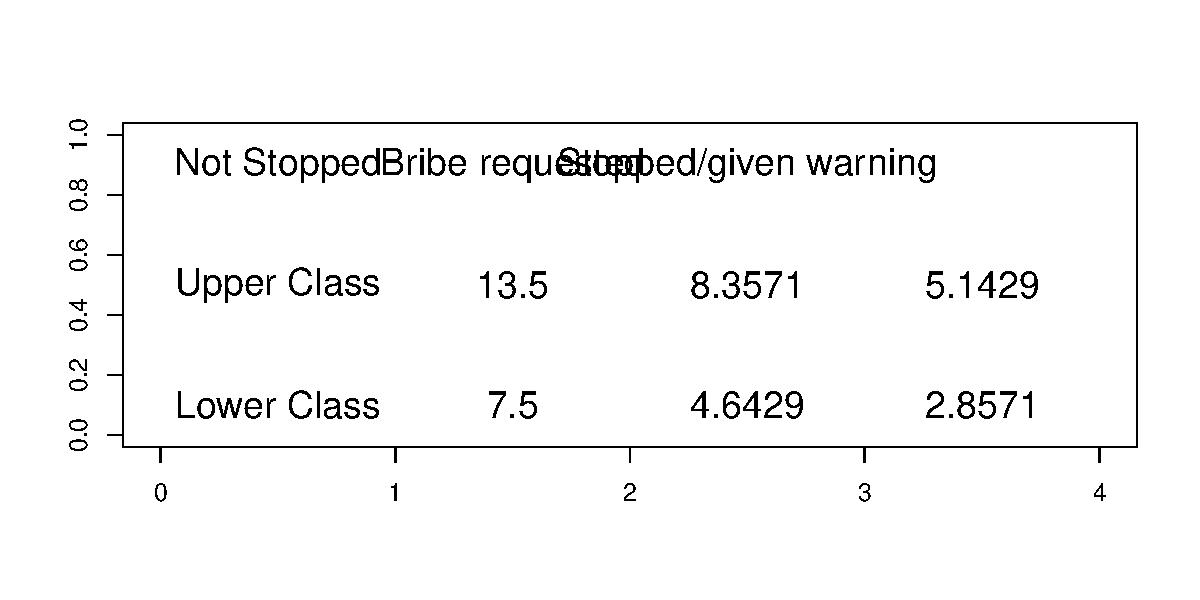
\includegraphics[width=.75\textwidth]{Expected_frequencyP02AF.pdf}
	\end{figure}
	
	\begin{table}[!htbp] \centering 
		\caption{} 
		\label{} 
		\begin{tabular}{@{\extracolsep{5pt}} cccc} 
			\\[-1.8ex]\hline 
			\hline \\[-1.8ex] 
			& Not Stopped & Bribe requested & Stopped/given warning \\ 
			\hline \\[-1.8ex] 
			Upper Class & $13.500$ & $8.357$ & $5.143$ \\ 
			Lower Class & $7.500$ & $4.643$ & $2.857$ \\ 
			\hline \\[-1.8ex] 
		\end{tabular} 
	\end{table} 
	
	
	Chi Squared Statistic
	
\begin{table}[!htbp] \centering 
	\caption{} 
	\label{} 
	\begin{tabular}{@{\extracolsep{5pt}} cccc} 
		\\[-1.8ex]\hline 
		\hline \\[-1.8ex] 
		& Not Stopped & Bribe requested & Stopped/given warning \\ 
		\hline \\[-1.8ex] 
		Upper Class & $0.018$ & $0.665$ & $0.671$ \\ 
		Lower Class & $0.033$ & $1.197$ & $1.207$ \\ 
		\hline \\[-1.8ex] 
	\end{tabular} 
\end{table} 
	
	I sum all the chi squared statistic values to get my final answer 
	X2 test statistic = TOTALSUM(O-E)%^%2/E
	X2 = 3.79
	
	Degrees of Freedom
	DF = (Number of Rows -1)*(Number of Columns-1)
	DF = (2-1)*(3-1)
	DF = 2
	
	Pearson's Chi-squared test
	
	data:  Political Science
	X-squared = 3.7912, df = 2, p-value = 0.1502
	
\end{verbatim}
	
	\item [(b)]
	Now calculate the p-value from the test statistic you just created (in \texttt{R}).\footnote{Remember frequency should be $>$ 5 for all cells, but let's calculate the p-value here anyway.}  What do you conclude if $\alpha = 0.1$?\\
	
	Assuming I did not get p value using the R code: chi-sq-result <- chisq.test(Political-Science)
	I can replace the values of chisq and DF into my formula p value = 1-P%(%X2<=X2%)%
	Where my X-suared is 3.7912, if I go to my statistic table I can see the following number:
	as my df is 2 and my significance level is 0.1 I have 4.610
	Now my formula looks like this p value = 1-P%(%3.7912<=4.610%)%
	On R will be P-value <- 1-pchisq(3.7912, df = 2)
	p-value = 0.1502
	
	if $\alpha = 0.1$ then I will fail to reject my null hypothesis. I do not have enough evidence to conclude that there is a significant 
	linear relationship between my variables. My p-value is 0.1502 is greater than my significance level 0.1. 
	
	In this research, we are interested to see if officers were more or less likely to solicit a bribe from drivers depending on their
	social class. 
	
	Null Hypothesis HO: There is no association between the driver's social class and the likelihood of officers soliciting a bribe. In other words, social class and bribe solicitation are independent.
	
	Alternative Hypothesis H1: There is an association between the driver's social class and the likelihood of officers soliciting a bribe. Social class and bribe solicitation are not independent.
	
	As I fail to reject my null hypothesis, it means that the data does not provide sufficient evidence to conclude that there is a significant association between social class and bribe solicitation. 


	
	\newpage
	\item [(c)] Calculate the standardized residuals for each cell and put them in the table below.
	\vspace{1cm}
	
	\begin{verbatim}
		
	\begin{table}[!htbp]
		\centering
		\caption{}
		\begin{tabular}{@{\extracolsep{5pt}} cccc}
			\hline
			\hline
			& Not Stopped & Bribe requested & Stopped/given warning \\
			\hline
			Upper Class & 0.322 & -1.642 & 1.523 \\
			Lower Class & -0.322 & 1.642 & -1.523 \\
			\hline
		\end{tabular}
	\end{table}
	
	
	
\end{verbatim}
	
	\vspace{7cm}
	\item [(d)] How might the standardized residuals help you interpret the results?  
	
	It helps me to identify outliers (I can identify data points that are far from the mean)
	A larger absolute value suggests a stronger deviation from what would be expected by random chance.
	The positive or negative sign tells me the direction of the deviation. In our dataset 
	Upper Class not stopped and Stopped/given warning is higher than we expected, same 
	with Lower Class Bribe requested. While Upper Class Bribe requested, Lower Class Not stopped
	and Stopped/given warning is lower than expected. 
	
	Conclusion: "Upper Class" individuals are significantly more likely to be in the "Stopped/given warning" category
	(large positive value) and significantly less likely to be in the "Bribe requested" category (large negative value)
	compared to what would be expected by random chance.
	
	"Lower Class" individuals are significantly more likely to be in the "Bribe requested" category (large positive value)
	and significantly less likely to be in the "Stopped/given warning" category (large negative value) compared to what
	would be expected by random chance.
	
	
	
\end{enumerate}
\newpage

\section*{Question 2: Economics}
Chattopadhyay and Duflo were interested in whether women promote different policies than men.\footnote{Chattopadhyay and Duflo. (2004). ``Women as Policy Makers: Evidence from a Randomized Policy Experiment in India. \textit{Econometrica}. 72 (5), 1409-1443.} Answering this question with observational data is pretty difficult due to potential confounding problems (e.g. the districts that choose female politicians are likely to systematically differ in other aspects too). Hence, they exploit a randomized policy experiment in India, where since the mid-1990s, $\frac{1}{3}$ of village council heads have been randomly reserved for women. A subset of the data from West Bengal can be found at the following link: \url{https://raw.githubusercontent.com/kosukeimai/qss/master/PREDICTION/women.csv}\\

\noindent Each observation in the data set represents a village and there are two villages associated with one GP (i.e. a level of government is called "GP"). Figure~\ref{fig:women_desc} below shows the names and descriptions of the variables in the dataset. The authors hypothesize that female politicians are more likely to support policies female voters want. Researchers found that more women complain about the quality of drinking water than men. You need to estimate the effect of the reservation policy on the number of new or repaired drinking water facilities in the villages.
\vspace{.5cm}
	

\newpage
\begin{enumerate}
	\item [(a)] State a null and alternative (two-tailed) hypothesis. 
	
	Null Hypothesis (Ho): The reservation policy has no effect on the number of new or repaired drinking water facilities in the village.
	
	Alternative Hypothesis (H1): The reservation policy has a significant effect on the number of new or repaired drinking water facilities in the villages.
	
	Significance level: .05
	
	\vspace{6cm}
	\item [(b)] Run a bivariate regression to test this hypothesis in \texttt{R} (include your code!).
	
	Please refer to R for code and step by step additionally you can find the manual calculation on tab 3 bivariate linear regression oo the excel file
	Because my p-value is 0.0197, which is less that my significance level of 0.05	I have enough evidence to reject my null hypothesis (H0)
	So, there is statistical evidence to suggest that the reservation policy has a significant effect on the number of new or repaired drinking water facilities in the villages.
	
	Note: If I had chosen a significance level of 0.01 it will be the opposite.
	
	\vspace{6cm}
	\item [(c)] Interpret the coefficient estimate for reservation policy. 
	
	First thing is to focus on the Intercept / Estimate which is 14.738, this is the estimated value of "water" when there is no policy
	The coefficient estimate for the reservation policy is 9.252. This means that, on average, villages with a reserved seat for women are expected to have 9.252 more new or 
	repaired drinking water facilities compared on villages without such a reservation, while holding all other variables constant. In other words, the reservation policy is 
	associated with a statistically significant increase in the number of these facilities in the villages.
	
	
\end{enumerate}

\end{document}
